% Table is required for multicolumn package with beamer
\documentclass[table]{beamer}

\usepackage{pucv_jz}


\title{Introducción}
\subtitle{Estadística Computacional}
\author[J.Z.O-2023]{Juan Zamora Osorio\\\url{juan.zamora@pucv.cl}}
\institute[PUCV]{Instituto de Estadística\\Pontificia Universidad Cat\'olica de Valpara\'iso}
%\date{\today}

\begin{document}

\frame{\titlepage}

%\begin{frame}
%\frametitle{Contents}
%\tableofcontents
%\end{frame}

% \section{Motivation}

%\begin{frame}
%\frametitle{Contents}
%\tableofcontents[currentsection]
%\end{frame}

\begin{frame}
    \frametitle{Probabilidades y estadística}
    \begin{block}{Filosofía / Epistemología}
        \begin{itemize}
            \item ¿Lo que sucede en el mundo depende del azar?
            \item ¿Qué es el azar?
        \end{itemize}
    \end{block}
    \begin{exampleblock}{Ejemplos}
        \begin{itemize}
            \item Un juego de azar.
            \item Máquinas de azar.
            \item Cuánto demora en responder una consulta web.
            \item El clima de mañana.
            \item Cuántas unidades de un producto se venden a través de un sitio web.
            \item Si un estudiante llega a la clase o no.
            \item Foto astronómica de estrellas lejanas.
            \item Partículas observadas en acelerador de partículas.
        \end{itemize}
    \end{exampleblock}
\end{frame}

\begin{frame}
    \frametitle{Probabilidades y estadística}
    \begin{block}{Filosofía / Epistemología}
        \begin{itemize}
            \item ¿Lo que sucede en el mundo depende del azar?
            \item ¿Qué es el azar?
        \end{itemize}
    \end{block}
    \begin{alertblock}{Pregunta}
        \begin{itemize}
            \item ¿Cuál es la diferencia entre \emph{azar}, \emph{aleatorio} y \emph{estocástico}?
        \end{itemize}
    \end{alertblock}
\end{frame}

\begin{frame}
    \frametitle{Probabilidades y estadística}
    \begin{alertblock}{Pregunta}
        \begin{itemize}
            \item ¿Cuál es la diferencia entre \emph{azar}, \emph{aleatorio} y \emph{estocástico}?
        \end{itemize}
    \end{alertblock}
    \begin{block}{Etimología}
        \begin{itemize}
            \item \emph{Azar} (castellano): De \emph{azzahr}, juego de dados, y éste del árabe \emph{zahr}, usado como \emph{dado} y que significa literalmente \emph{flores}.
            \item \emph{Aleatorio} (latín): De \emph{alea}, suerte, usado como sinónimo de juego de azar.
            \item \emph{Estocástico} (griego): De \emph{stokhastikos}, apuntar a un blanco, conjeturar, a su vez de \emph{stokhos}, el objetivo apuntado.
        \end{itemize}
    \end{block}
\end{frame}

\begin{frame}
    \frametitle{Probabilidades y estadística}
    \begin{alertblock}{Pregunta}
        \begin{itemize}
            \item ¿Cuál es la diferencia entre \emph{azar}, \emph{aleatorio} y \emph{estocástico}?
        \end{itemize}
    \end{alertblock}
    \begin{center}
        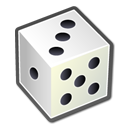
\includegraphics[height=0.4\textheight]{Nuvola_apps_atlantik}
        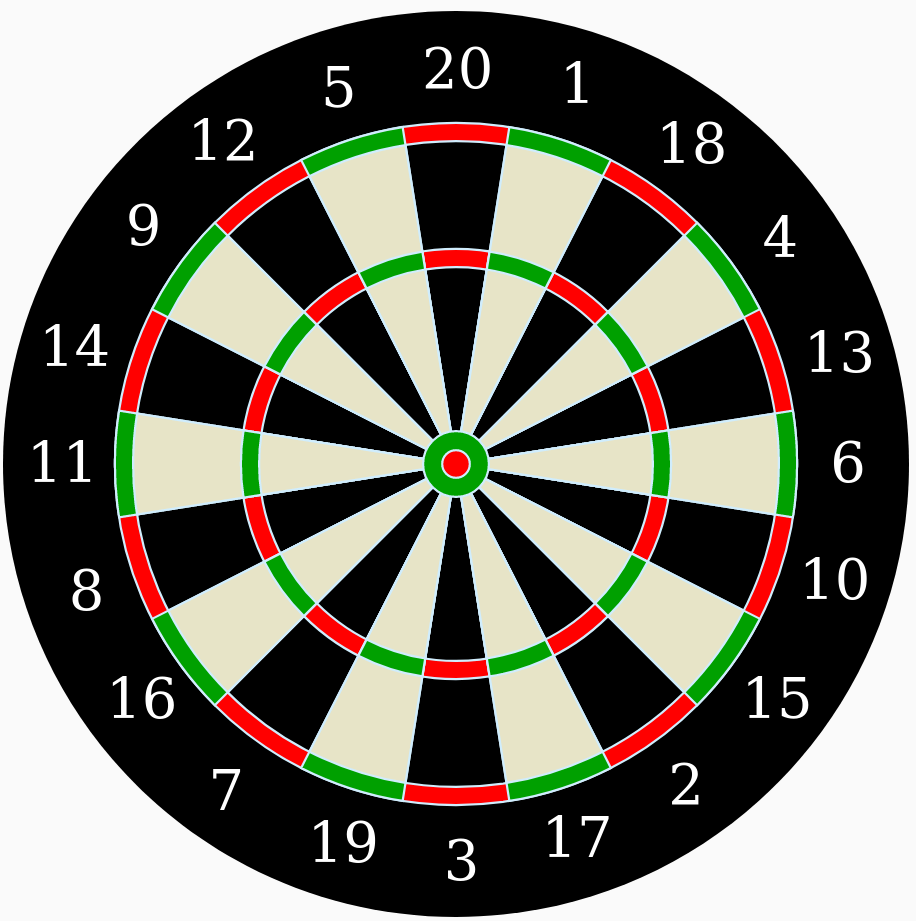
\includegraphics[height=0.4\textheight]{dartboard}
    \end{center}
    \begin{alertblock}{Entre dados y dardos}
        \begin{itemize}
            \item La diferencia no es solo una letra \emph{r}, sino una concepción de mundo diferente.
        \end{itemize}
    \end{alertblock}
\end{frame}

\begin{frame}
    \frametitle{Probabilidades}
    \begin{block}{Origen: Carneades, siglo II a.C.}
        \begin{itemize}
            \item Escéptico: No es posible conocer algo absolutamente.
            \item Propone que toda decisión (jurídica / política) tiene incertidumbre.
            \item Para funcionar de manera práctica, asignar un valor de verdad a las afirmaciones, asociado a seguridad que sujeto tiene de afirmación.
        \end{itemize}
    \end{block}
    \begin{center}
        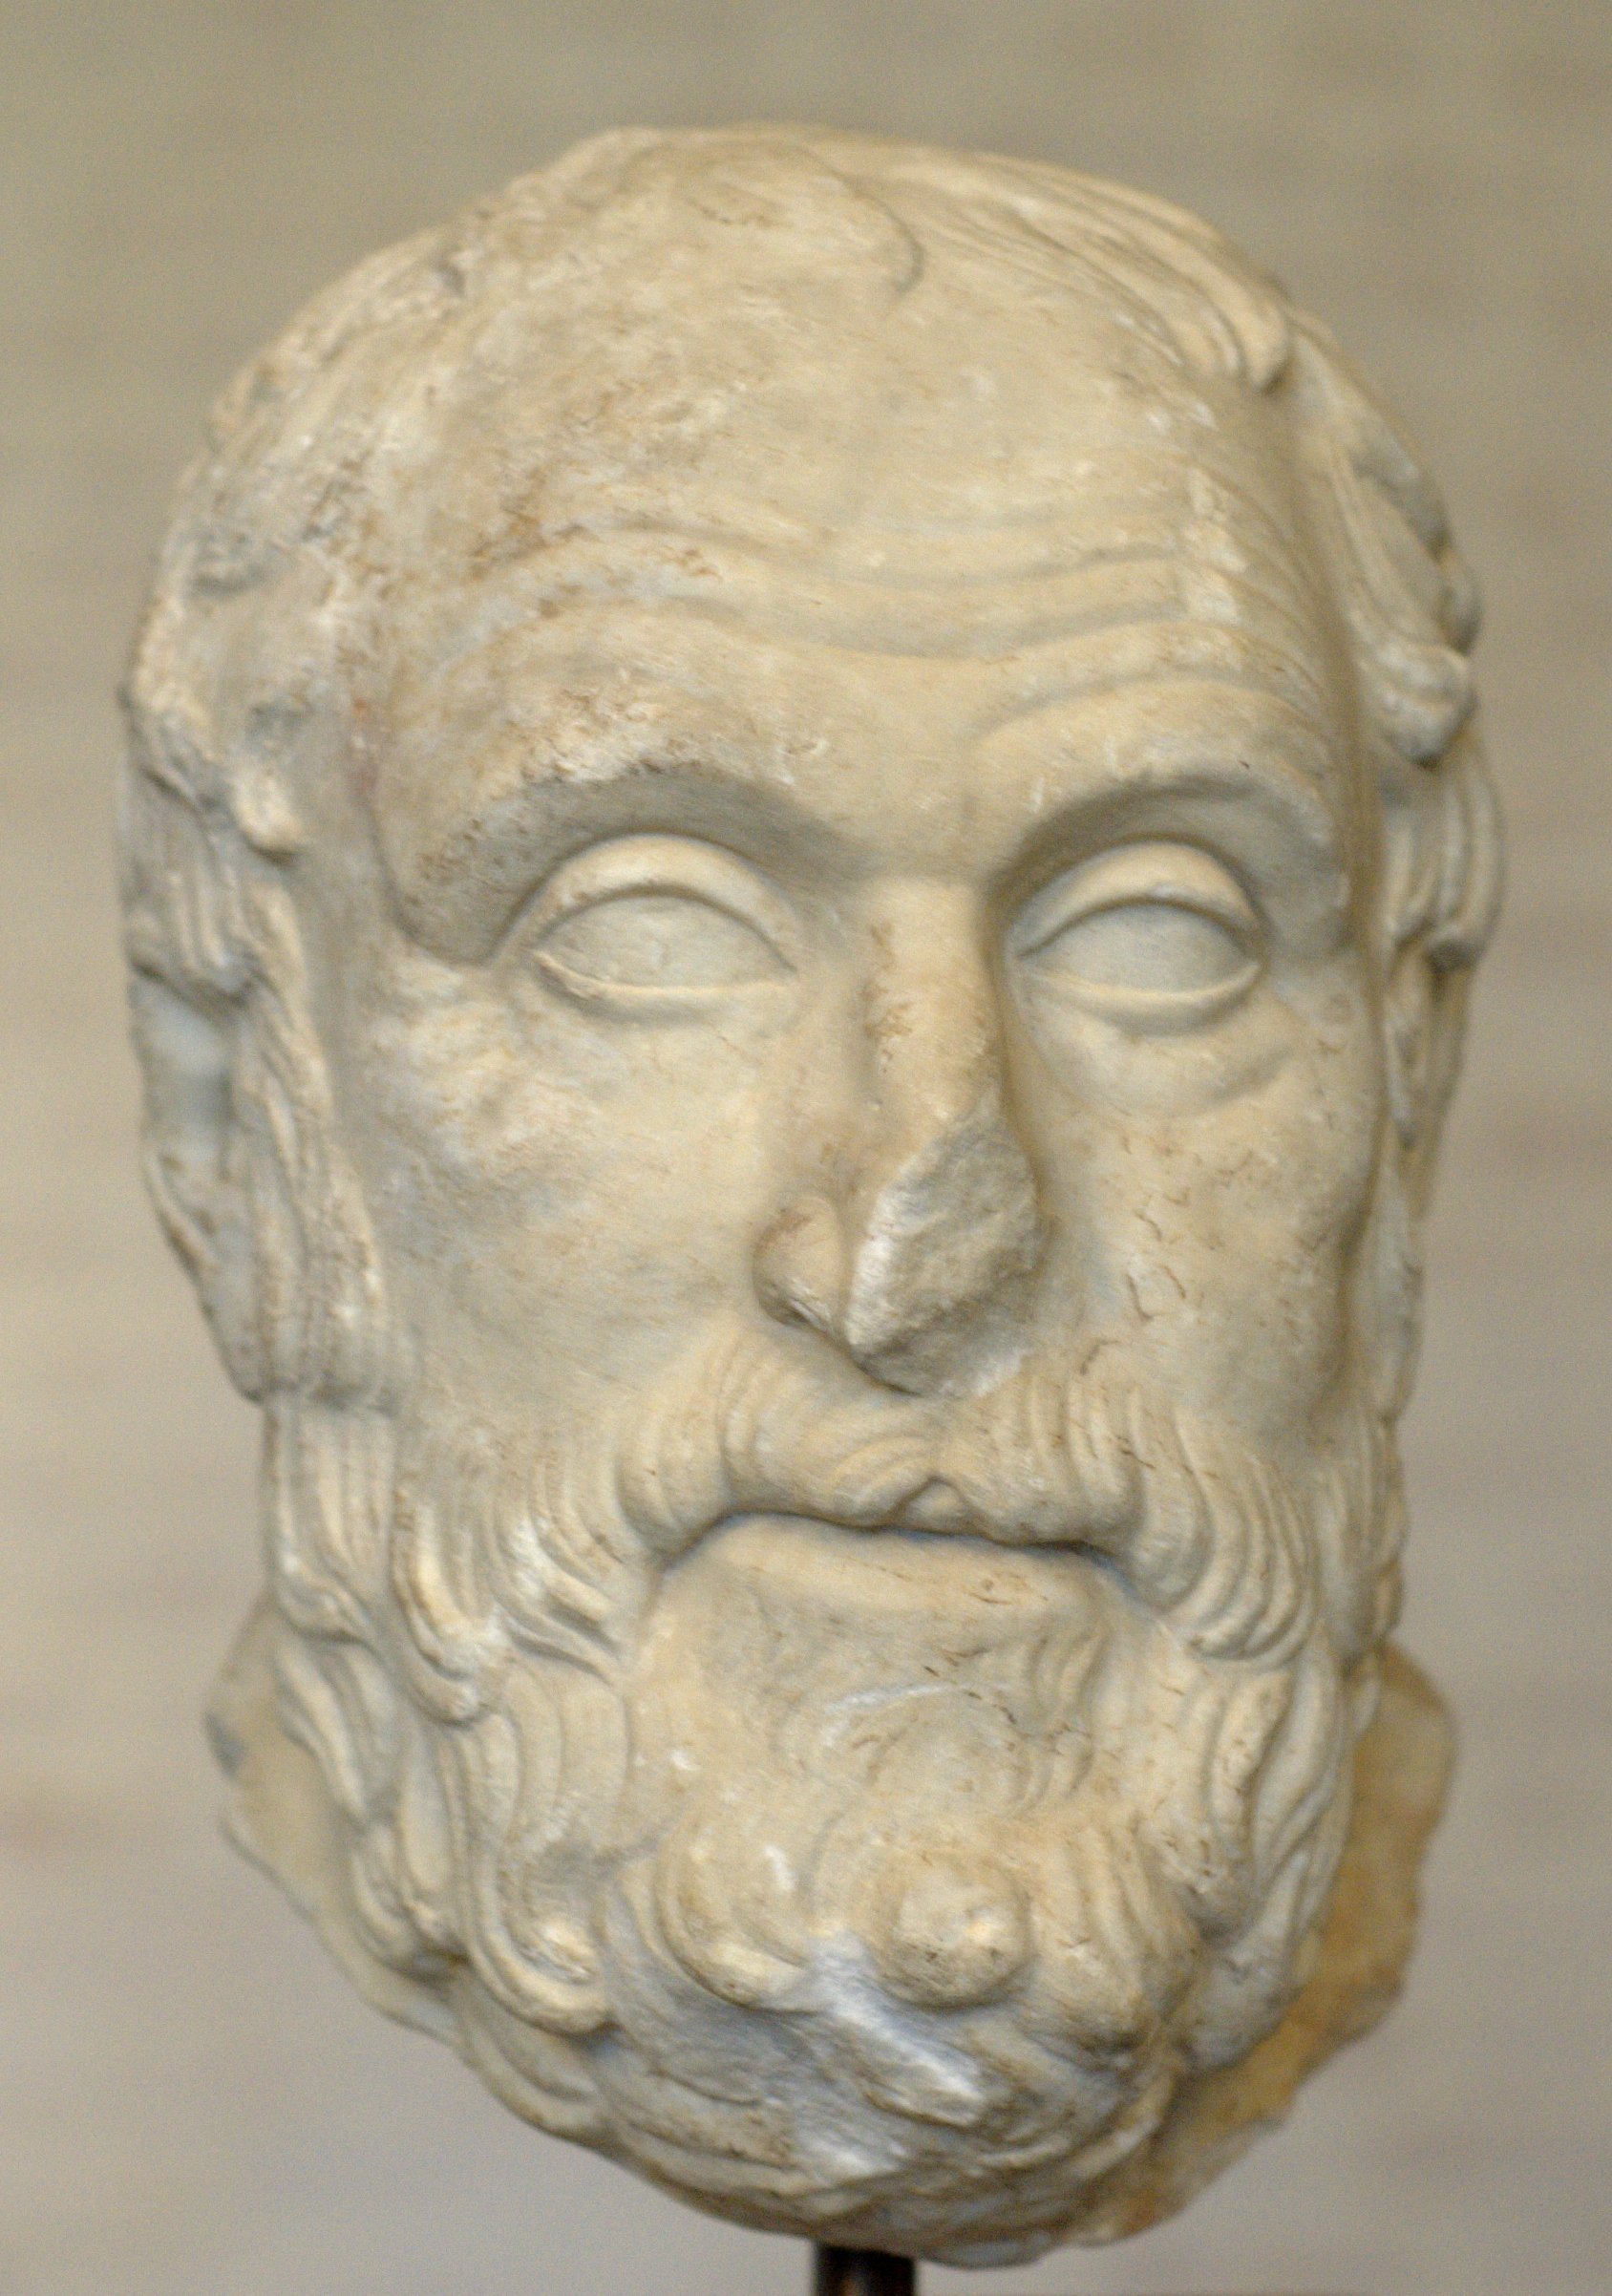
\includegraphics[height=0.4\textheight]{Head_Karneades_Glyptothek_Munich}
    \end{center}
\end{frame}

\begin{frame}
    \frametitle{Probabilidades}
    \begin{block}{Teoría de Probabilidades}
        \begin{itemize}
            \item Se interpreta como la modelación matemática del azar, ella debe dar cuenta del conocimiento acumulado por sobre los fenómenos del azar y sus leyes. La noción de probabilidad está subordinada a una determinada aproximación a los fenómenos del azar.
        \end{itemize}
    \end{block}
    \begin{block}{Actual: Andréi Kolmogórov (1930)}
        \begin{itemize}
            \item Teoría basada en el concepto matemático de medida, que explica al menos las tres primeras leyes del azar en diferentes contextos.
        \end{itemize}
    \end{block}

    \begin{tikzpicture}[remember picture, overlay]
    \node[above left , yshift=-0.1cm, xshift=-0.5cm] at (current page.south) 
    {
        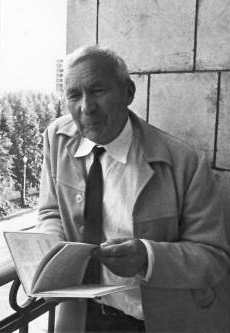
\includegraphics[width=0.15\textwidth]{Andrej_Nikolajewitsch_Kolmogorov}
    };
	\end{tikzpicture}
    
    
\end{frame}

\begin{frame}
    \frametitle{Probabilidades -- Leyes del azar}
    \begin{block}{Ley de los grandes números}
        \begin{itemize}
            \item Modelo matemático para comportamiento del promedio, permite construir visión frecuentista de la probabilidad.
        \end{itemize}
    \end{block}
    \begin{block}{Ley del comportamiento de las fluctuaciones}
        \begin{itemize}
            \item Estudio de las fluctuaciones de las pequeñas variaciones y sus correspondientes modelos matemáticos referidos a diferentes versiones del teorema del límite central.
        \end{itemize}
    \end{block}
    \begin{block}{Ley de la complejidad}
        \begin{itemize}
            \item La complejidad de todo sistema dinámico aumenta en el curso de su evolución (Boltzmann).
        \end{itemize}
    \end{block}
\end{frame}

\begin{frame}
    \frametitle{¿Qué es la estadística?}
    \begin{block}{Varias definiciones}
        \begin{itemize}
            \item Cómo opinar y tomar decisiones bajo la presencia de incertidumbre.
            \item Ciencia y arte de tomar decisiones basadas en evidencia cuantitativa.
            \item Colección de métodos que nos ayudan a describir, resumir, interpretar y analizar datos.
        \end{itemize}
    \end{block}
    \begin{alertblock}{}
        \begin{itemize}
            \item Sin incertidumbre, ¿hay necesidad de métodos estadísticos?
        \end{itemize}
    \end{alertblock}
\end{frame}

\begin{frame}
    \frametitle{¿Qué es la estadística?}
    \begin{block}{Historia}
        \begin{itemize}
            \item Proviene de la ciencia política de recolectar datos para describir poblaciones, negocios, etc. para administrar un estado.
            \item Siglo XIX se amplía para diseñar y análizar experimentos en agricultura.
            \item Siglo XX se amplía a industrias.
            \item Siglo XXI: ciencia de datos.
        \end{itemize}
    \end{block}
    \begin{block}{¿Dónde se utiliza?}
        \begin{itemize}
            \item Casi en todas las áreas del conocimiento que recolectan e interpretan datos.
            \item Transformar datos en información.
        \end{itemize}
    \end{block}
\end{frame}

\begin{frame}
    \frametitle{Estadística y computación}
    \begin{block}{Explosión de datos}
        \begin{itemize}
            \item Vivimos en una sociedad inundada de datos.
            \item Bioinformática, astronomía, física, medio ambiente, finanzas, comercio, reconocimiento de voz, vigilancia, fotos, etc.
            \item Ley de Kryder: cantidad de datos se duplica cada 12-14 meses.
        \end{itemize}
    \end{block}

    
    
    \begin{tikzpicture}[remember picture, overlay]
    \node[above left , yshift=0.5cm, xshift=-0.5cm] at (current page.south) 
    {
        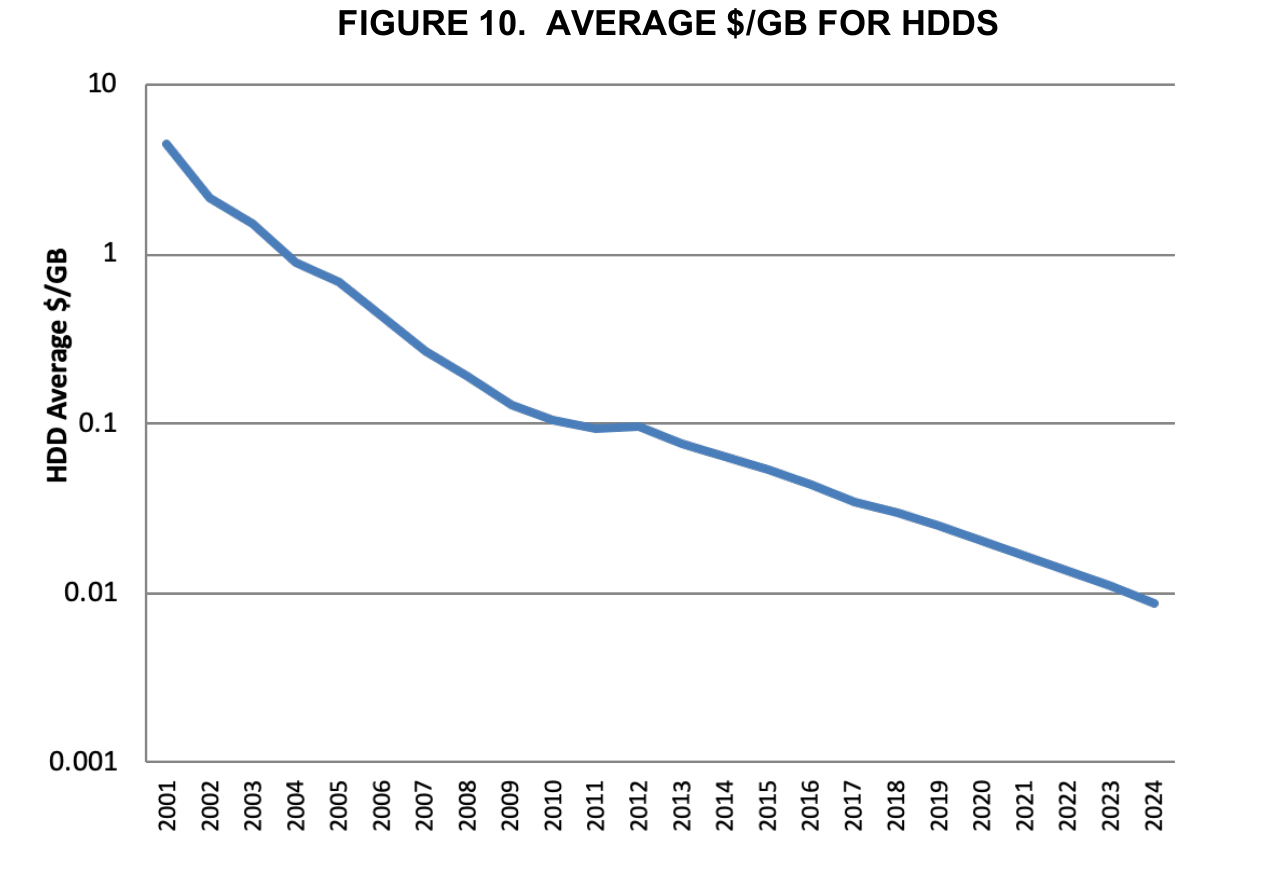
\includegraphics[height=0.35\textheight]{KrydersLaw}
    };
    \node[above left , yshift=0.5cm, xshift=4.5cm] at (current page.south) 
    {
        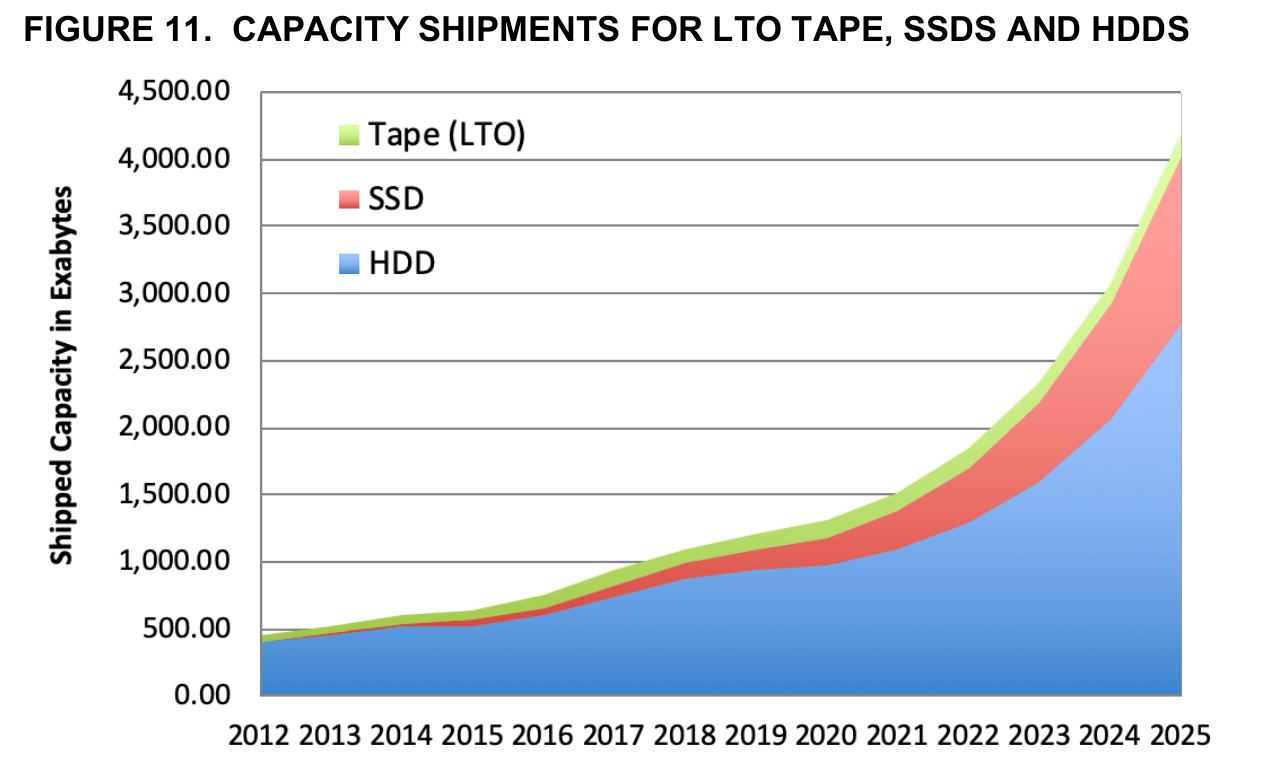
\includegraphics[height=0.35\textheight]{krydersExabytesShipped}
    };    
	\end{tikzpicture}
    
\end{frame}

\begin{frame}
    \frametitle{Estadística y computación}
    \begin{block}{Computación}
        \begin{itemize}
            \item Procesar dichos datos y extraer valor es fundamental.
            \item Volumen requiere algoritmos y competencias en computación.
            \item Algoritmos probabilísticos.
        \end{itemize}
    \end{block}
    \begin{block}{Gran diferencia}
        \begin{itemize}
            \item Aprender a vivir con datos que tienen errores.
            \item \emph{El conocimiento estadístico es fundamental.}
        \end{itemize}
    \end{block}
\end{frame}

\begin{frame}
    \frametitle{Estadística}
    \begin{block}{Matemáticas}
        \begin{itemize}
            \item En matemáticas muchos problemas tienen una respuesta única y en que estamos todos de acuerdo.
            \item ¡Se requieren supuestos que pueden llegar a conclusiones diferentes!
        \end{itemize}
    \end{block}
    \begin{block}{Otras disciplinas -- \emph{``Arte''}}
        \begin{itemize}
            \item Parte del trabajo es identificar el problema para poder usar las herramientas matemáticas.
            \item Se requiere conocer el área de estudio.
            \item Experiencia y creatividad.
        \end{itemize}
    \end{block}
    \end{frame}
    \begin{frame}
    \frametitle{Estadistica}
    \begin{block}{Comunicación}
        \begin{itemize}
            \item Cómo presentar resultados a clientes.
            \item Cómo comunicar incertidumbre.
            \item Cómo comunicar riesgo.
        \end{itemize}
    \end{block}
\end{frame}

\begin{frame}
    \frametitle{Ciencia de datos (\emph{data science})}
    \begin{block}{Intersección multidisciplinaria}
        \begin{itemize}
            \item Computación y aprendizaje automático (\emph{Machine Learning}).
            \item Estadística.
            \item Dominio de aplicación.
        \end{itemize}
    \end{block}
\end{frame}

\begin{frame}
    \frametitle{Análisis estadístico}
    \begin{block}{Partes}
        \begin{itemize}
            \item Recolección de datos.
            \item Administración de los datos.
            \item Aplicación de procedimientos estadísticos.
            \item Interpretación de los resultados.
        \end{itemize}
    \end{block}
    \begin{block}{Este curso}
        \begin{itemize}
            \item Nos concentraremos en las dos últimas.
            \item \emph{¡Todas son importantes!}
        \end{itemize}
    \end{block}
\end{frame}

\begin{frame}
    \frametitle{Análisis estadístico}
    \begin{block}{Tipos}
        \begin{itemize}
            \item Descriptivo.
            \item Predictivo.
            \item Causalidad.
        \end{itemize}
    \end{block}
    \begin{center}
        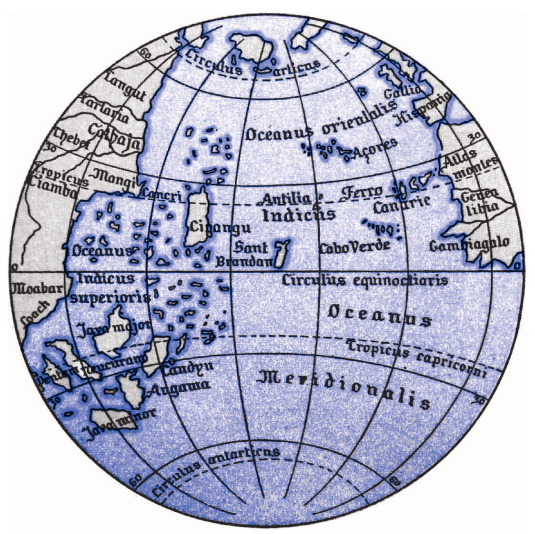
\includegraphics[height=0.5\textheight]{sr_smallworld}
    \end{center}
\end{frame}

\begin{frame}
    \frametitle{Análisis estadístico}
    \begin{block}{Tipos}
        \begin{itemize}
            \item Descriptivo.
            \item Predictivo.
            \item Causalidad.
        \end{itemize}
    \end{block}
    \begin{center}
        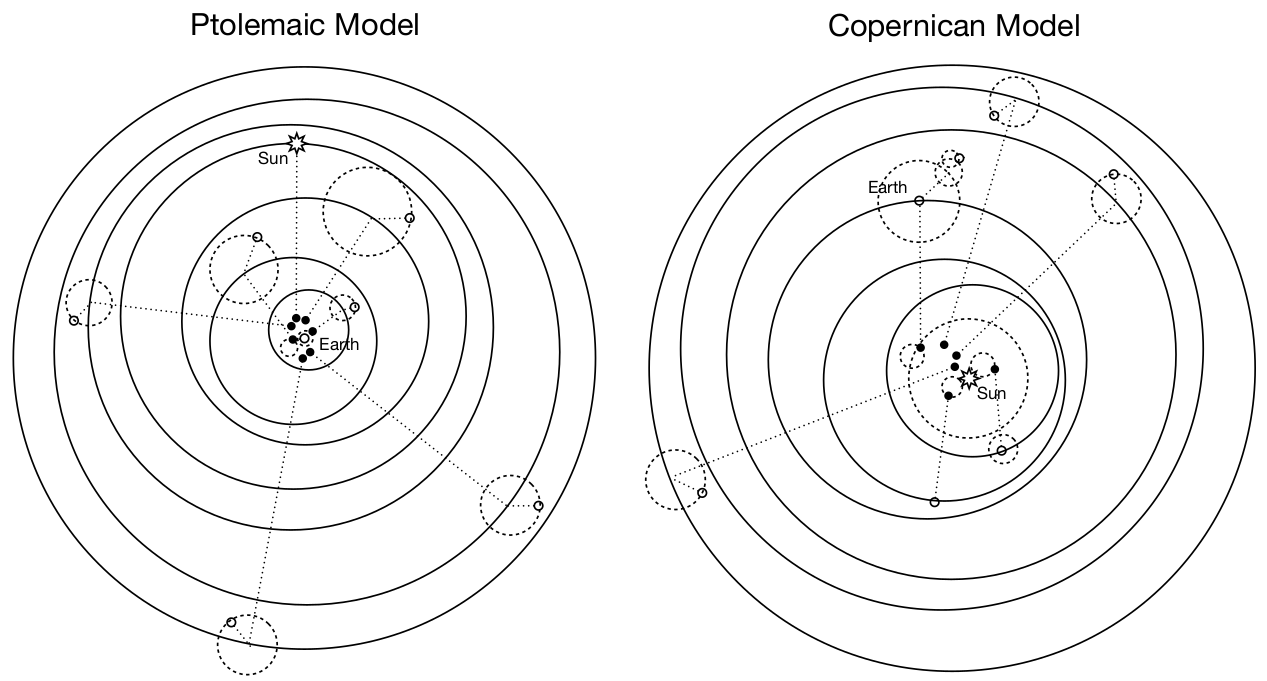
\includegraphics[height=0.5\textheight]{sr_copernico}
    \end{center}
\end{frame}

\begin{frame}
    \frametitle{Probabilidades e inferencia estadística}
    \begin{center}
        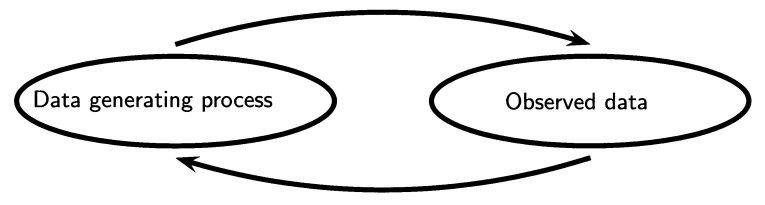
\includegraphics[height=0.3\textheight]{all2014_probabilidad_vs_inferencia}
    \end{center}
    \begin{block}{Probabilidades}
        \begin{itemize}
            \item ¿Dado un proceso que genera datos, cuáles son las propiedades que observaremos?
        \end{itemize}
    \end{block}
    \begin{block}{Inferencia estadística}
        \begin{itemize}
            \item ¿Dadas las observaciones, qué podemos decir sobre el proceso que genera los datos?
        \end{itemize}
    \end{block}
\end{frame}

\begin{frame}
    \frametitle{Enlaces útiles -- Conjuntos de datos}
    \begin{block}{Internacionales}
        \begin{itemize}
            \item Kaggle: \url{https://www.kaggle.com/datasets}.
            \item Google: \url{https://datasetsearch.research.google.com/}.
            \item Google: \url{https://www.google.com/publicdata}.
            \item UCI: \url{https://archive.ics.uci.edu/ml/datasets.php}.
        \end{itemize}
    \end{block}
\end{frame}

\begin{frame}
    \frametitle{Enlaces útiles -- Conjuntos de datos}
    \begin{block}{Nacionales}
        \small
        \begin{itemize}
            \item Instituto Nacional de Estadísticas: \url{https://ine.cl/}.
            \item Dirección Meteorológica de Chile: \url{https://climatologia.meteochile.gob.cl/}.
            \item Banco Central: \url{https://www.bcentral.cl/inicio}.
            \item Centro Sismológico Nacional: \url{https://www.sismologia.cl/index.html}.
            \item Infraestructura de Datos Geoespaciales de Chile: \url{https://www.ide.cl/}.
            \item Estadísticas Servicio de Impuestos Internos: \url{https://www.sii.cl/destacados/ogp/index.html}.
            \item Biblioteca del Congreso Nacional: \url{https://www.bcn.cl/leychile/}.
            \item Coordinador Eléctrico Nacional: \url{https://www.coordinador.cl/}.
            \item Energía Maps: \url{https://energiamaps.cne.cl/}.
            \item Carabineros: \url{https://stop.carabineros.cl/}.
        \end{itemize}
    \end{block}
\end{frame}

\begin{frame}
    \frametitle{Enlaces útiles -- Libros}
    \begin{block}{}%Libros}
        \begin{itemize}
            %\item \textbf{All of Statistics: A concise course in statistical inference}. Springer, 2004. Larry Wasserman.
            %\item \textbf{A modern introduction to probability and statistics: Understanding why and how}. Springer, 2005. F. M. Dekking, C. Kraaikamp, H. P. Lopuha\"a, L. E. Meester.
            %\item \textbf{Introductory statistics with R}. Springer, 2008. Peter Dalgaard.
            %\item \textbf{Data Analysis: Statistical and computational methods for scientists and engineers}. Springer, 2014. Siegmund Brandt.
            \item \textbf{Information theory, inference and learning algorithms}. Cambridge university press, 2003. David J. C. MacKay.% \url{https://www.inference.org.uk/mackay/itila/}.
            \item \textbf{Probability \& Statistics for Engineers \& Scientists}. Pearson Education, 2012. Ronald E. Walpole, Raymond H. Myers, Sharon L. Myers, Keying Ye.
            \item \textbf{Probability \& Statistics for Engineering and the Sciences}. Cengage Learning, 2015. Jay L. Devore.
            \item \textbf{Introduction to Statistics and Data Analysis}. Springer, 2016. Christian Heumann, Michael Schomaker Shalabh.% \url{https://chris.userweb.mwn.de/book/}.
            \item \textbf{Probability and Statistics for Computer Science}. UK: Springer International Publishing, 2018. David Forsyth.
          
        \end{itemize}
    \end{block}
\end{frame}

\begin{frame}
\frametitle{Enlaces útiles}
\begin{itemize}
  \item \textbf{Statistical rethinking: A Bayesian course with examples in R and Stan}. Chapman and Hall/CRC, 2018. Richard McElreath.% \url{https://xcelab.net/rm/statistical-rethinking/}.
           \item \textbf{Applied Multivariate Statistical Analysis}. Springer Nature, 2019. Wolfgang Karl H\"ardle, L\'eopold Simar.
\end{itemize}         
    \begin{block}{Otros cursos}
        \begin{itemize}
            \item \textbf{Probabilidad y Estadística USM}. Ronny Vallejos. \url{https://www.youtube.com/playlist?list=PLRdsr8w_wLNzYYSYP6bvf1p30mo27X9q-}.
            \item \textbf{Pensamiento estadístico}. Felipe Bravo-Marquez. \url{https://github.com/dccuchile/CC6104}.
        \end{itemize}
    \end{block}
\end{frame}

\iffalse
\begin{frame}[allowframebreaks, noframenumbering]
\frametitle<presentation>{References}
\printbibliography
%\bibliographystyle{apalike}
\end{frame}
\fi

\end{document}
